\section{Feature Engineering}
\label{sec:chapter_4_feature_engineering}
\begin{itemize}
	\item Create useful features from temporal data
\end{itemize}
\subsection{Time Domain}
\begin{itemize}
	\item Summarize values of a certain attributes in a window size of $\lambda$ steps before. If we would take the time steps $t$ and $t-1$ into account, our value for $\lambda$ is $1$
	\item Note that we cannot compute any values for the time steps $t=1,..,\lambda$.
\end{itemize}
\subsubsection{Numerical}
\begin{itemize}
	\item Aggregate values by mean, min, max, stddev, etc. (including current time step)
	\item We could also use coefficient between first and last value interpolation (gradient of attribute)
\end{itemize}
\subsubsection{Categorical}
\begin{itemize}
	\item Generate patterns of occurrences of categorical values. We distinguish between successive \texttt{(b)} and co-occurring \texttt{(c)} actions/classes. Example patterns:
	\begin{itemize}
		\item Activity level = high \texttt{(c)} Activity = running
		\item Activity = running \texttt{(b)} Activity = running
	\end{itemize}
	\item If we have a window size of $\lambda$, we just see if there is any time step within $t-\lambda, ..., t-1, t$ where the activities are co-occuring \texttt{(c)}, or there is one activity happening (arbitrary number of time steps) before another \texttt{(b)}.
	\item We can find important patterns by determining the support of such. This is important as the number of patterns exponentially increases with the number of categories/attributes, and only frequent patterns are interesting.
	\item The support of a pattern is defined as the proportion of the processed time steps at which this pattern would occur.
	\item The algorithm for finding such patterns starts with single attribute patterns, and extends only those which have sufficient support. In the end, we add all patterns (including the single-attribute) with enough support.
	\begin{figure}[ht!]
		\centering
		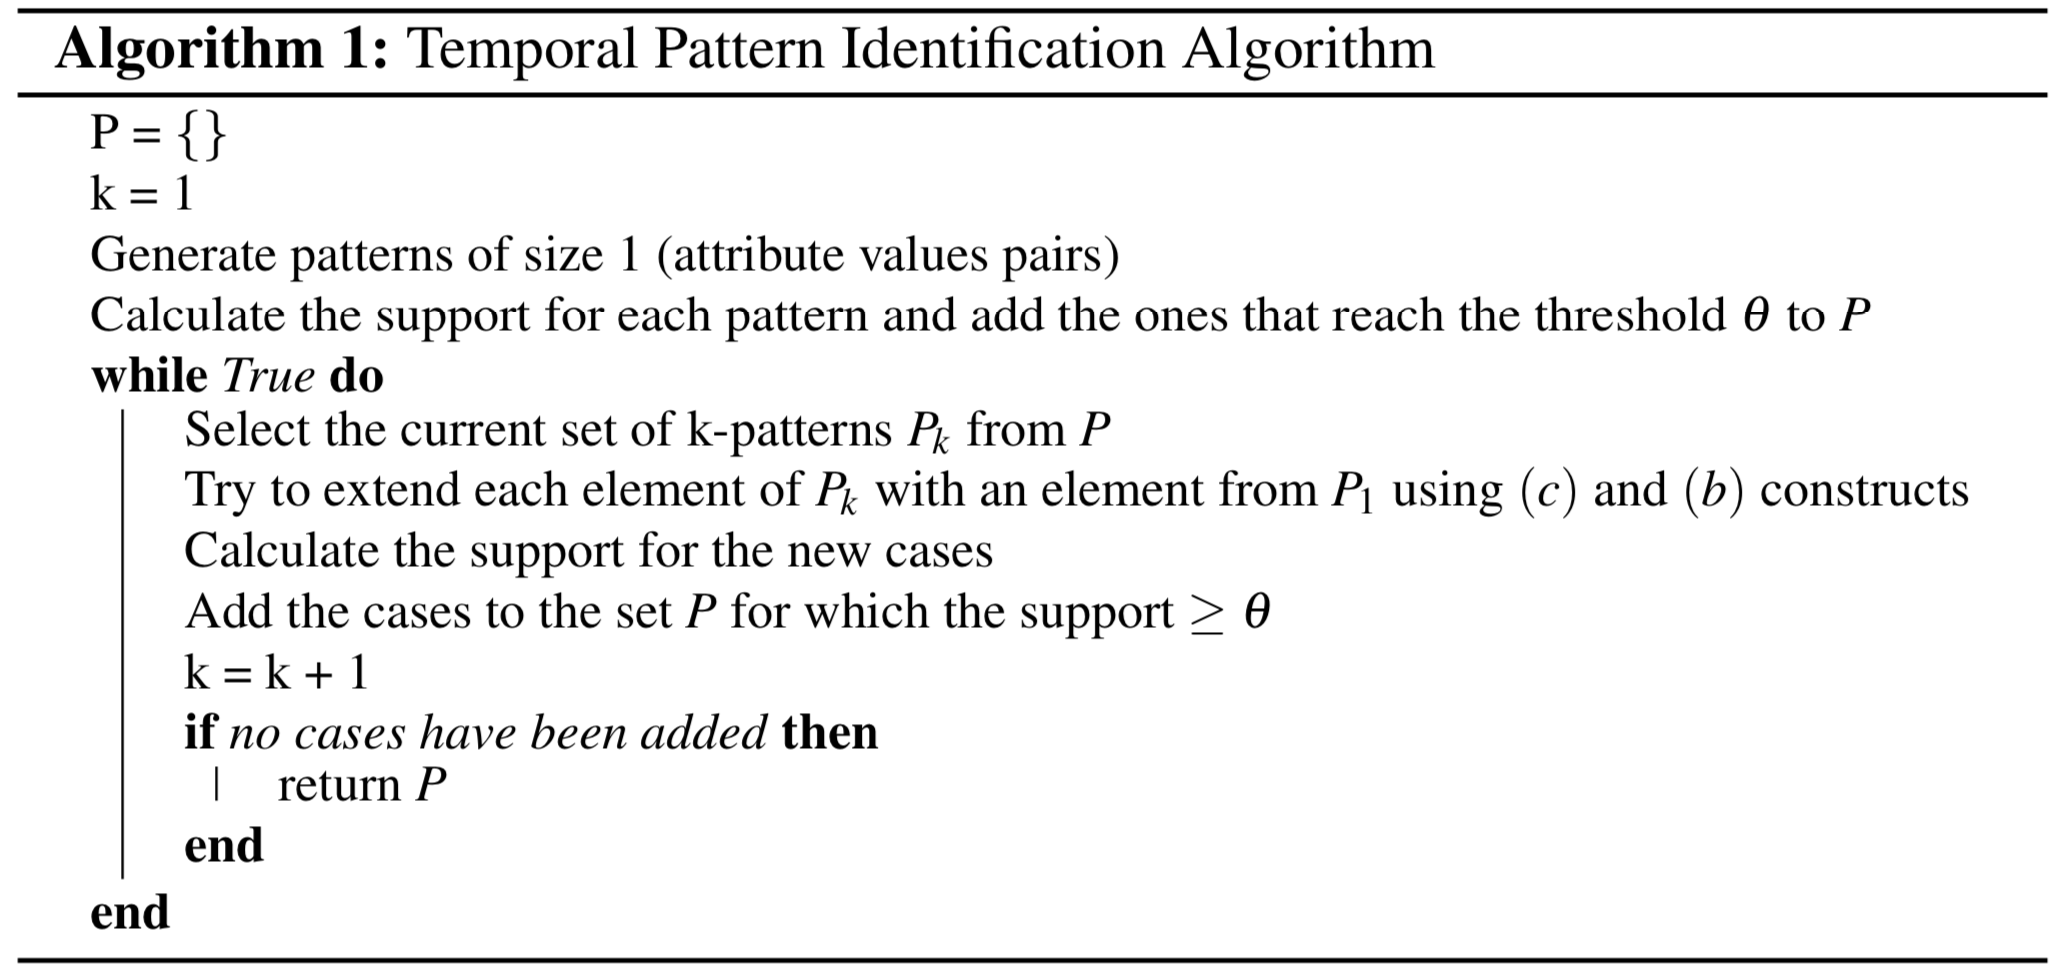
\includegraphics[width=0.5\textwidth]{figures/chapter_4_pattern_identification.png}
		\caption{Pattern identification algorithm}
	\end{figure}
\end{itemize}
\subsubsection{Mixed data}
\begin{itemize}
	\item We can also combine numerical and categorical attributes for features
	\item Hereby, we create categories from numerical data by looking at them \textbf{qualitatively} (greetings from QR). For example, we can define ranges like low, medium and high, or look at the trend/gradients as \textit{increasing} or \textit{decreasing}
	\item Afterwards, we can apply the categorical approach on those
\end{itemize}
\subsection{Frequency Domain}
\begin{itemize}
	\item Apply Fourier transformation on data within a window of $\lambda$ (plus the current time point $t$) to extract periodicity of the data
	\item Assume a base frequency of $f_0 = \frac{2\pi}{\lambda+1}$ (or $f_0 = \frac{N_{\text{sec}}}{\lambda+1}$ in seconds) which is the lowest frequency with a complete sinusoid in it. 
	\item We look at all the frequencies $\left\{0\cdot f_0, 1\cdot f_0, ..., \lambda \cdot f_0\right\}$ and determine the corresponding amplitudes
	\item Our features can be:
	\begin{itemize}
		\item Frequency with highest amplitude
		\item Frequency-weighted signal average $\frac{\sum_{k=0}^{\lambda} a_{t-\lambda}^{t}(k) \cdot f(k)}{\sum_{k=0}^{\lambda} a_{t-\lambda}^{t}(k)}$
		\item \textit{Power Spectrum Entropy}: Amount of information in the signal
		$$x\_pse = - \sum_{k=0}^{\lambda} p_{t-\lambda}^{t}(k) \ln p_{t-\lambda}^{t}(k), \hspace{3mm}\text{with}\hspace{2mm} p_{t-\lambda}^{t}(k) = \frac{|a_{t-\lambda}^{t}(k)|^2}{\sum_{i=0}^{\lambda} |a_{t-\lambda}^{t}(i)|^2}$$
	\end{itemize}
\end{itemize}
\subsection{Unstructured data}
\begin{itemize}
	\item How to handle non-temporal/unstructured data like text, audio, images, etc.
	\item Here we focus on text. The standard pipeline contains for steps:
	\begin{itemize}
		\item \textit{Tokenization}: split sentence into smallest parts 
		\item \textit{Lower case}: put all words to lower case to have no difference in such
		\item \textit{Stemming}: reduce words to their stem to remove all small variations (like tense, etc.)
		\item \textit{Stop word removal}: remove known, uninformative stop words 
	\end{itemize}
	\begin{figure}[ht!]
		\centering
		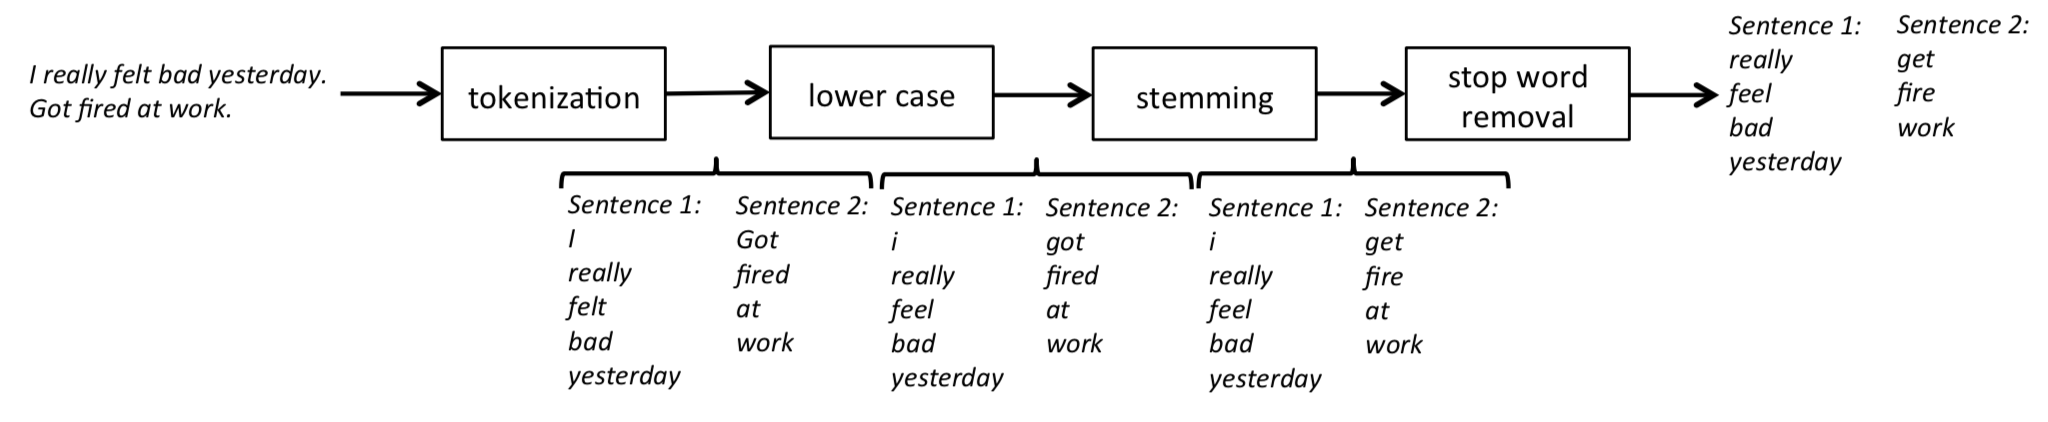
\includegraphics[width=0.5\textwidth]{figures/chapter_4_text_pipeline.png}
		\caption{Pipeline of text processing}
	\end{figure}
	\item Three approaches in general
	\begin{itemize}
		\item \textbf{Bag of words}: count occurrences of n-gram within text. These counts are the features for the text
		\item \textbf{TF-IDF}: BoW does not take ``uniqueness'' of word into account. Thus, TF-IDF takes occurrences of a word in a text and in the whole corpus into account
		\item \textbf{Topic modeling}: assume that any text is a combination of $k$ topics. Perform LDA to get these topics, and topic distribution of text is its features.
	\end{itemize}
\end{itemize}